\chapter{Wprowadzenie}
\label{cha:wprowadzenie}

\section{Joł}

Praca

\begin{figure}[h]
    \centering
    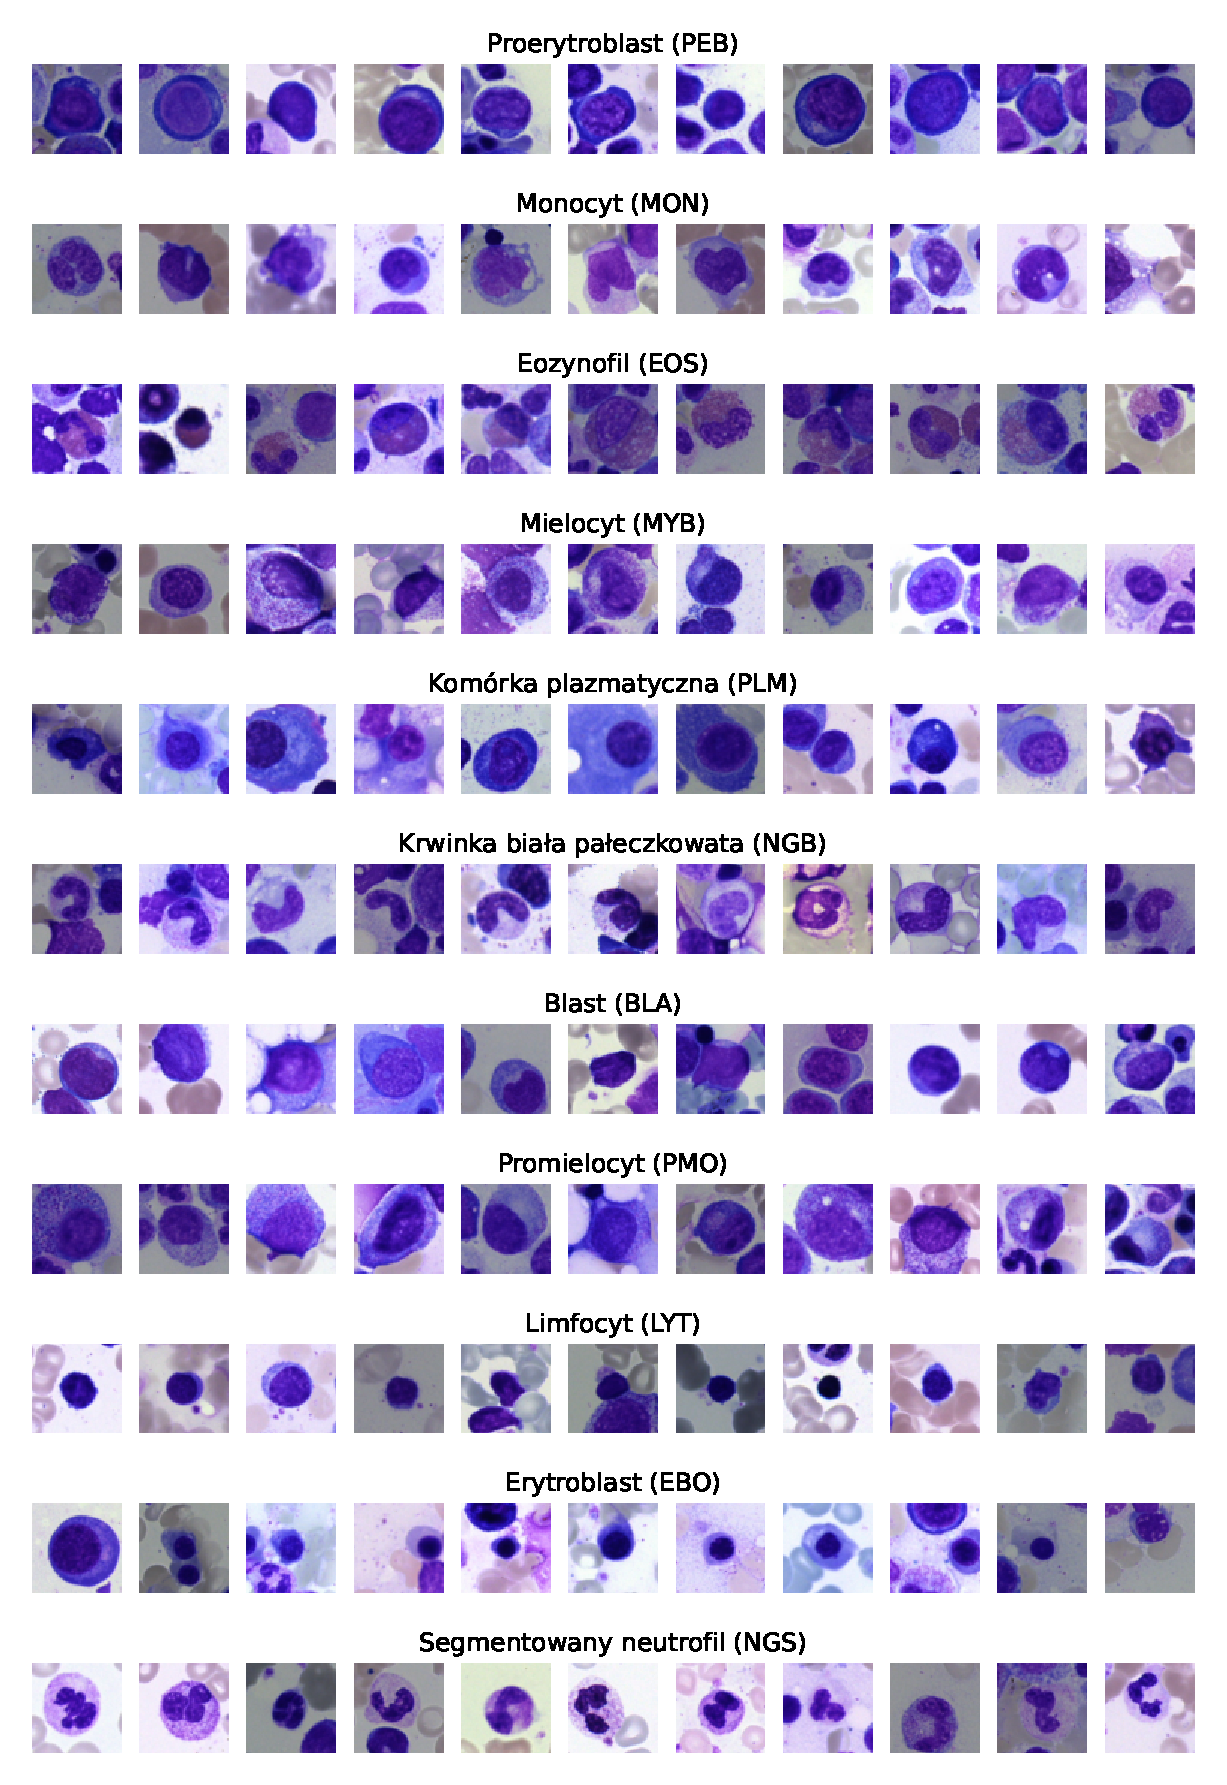
\includegraphics[width=0.1\textwidth]{images_examples}
    \caption{Test}
\end{figure}


\section{Cele pracy}
\label{sec:celePracy}

Celem poniższej pracy jest

\subsection{Jakiś tytuł 2}

\section{Zawartość pracy}
\label{sec:zawartoscPracy}

W rozdziale~\ref{cha:wprowadzenie} przedstawiono podstawowe informacje dotyczące struktury dokumentów w \LaTeX u. Alvis~\cite{Alvis2011} jest językiem\textellipsis

Jeszcze kilka odnośników do bibliografii~\cite{Resnetx}.